\documentclass{article}

\usepackage{graphicx}
\usepackage{color}
\usepackage{tikz}
\usepackage{pgfplots}
% \usepackage{pgf-umlsd}
\usepackage{ifthen}

\pgfplotsset{compat=1.7}
\pgfrealjobname{survey}
\begin{document}
\beginpgfgraphicnamed{hanoitower}
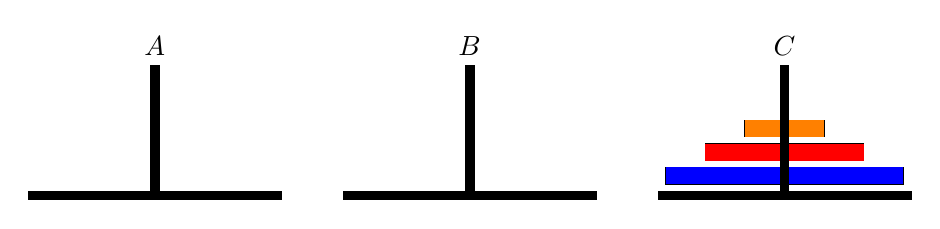
\begin{tikzpicture}[scale=1]
  % \draw[use as bounding box, transparent] (-1.8,-1.8) rectangle (17.2, 3.2);

  % Define the macro.
  % 1st argument: Height and width of the layer rectangle slice.
  % 2nd argument: Depth of the layer slice
  % 3rd argument: X Offset --> use it to offset layers from previously drawn layers.
  % 4th argument: Options for filldraw.
  % 5th argument: Text to be placed below this layer.
  % 6th argument: Y Offset --> Use it when an output needs to be fed to multiple layers that are on the same X offset.

  \newcommand{\networkLayer}[6]{
    \def\a{#1} % Used to distinguish input resolution for current layer.
    \def\b{#2}
    \def\c{#3} % Width of the cube to distinguish number of input channels for current layer.
    \def\d{#4} % X offset for current layer.
    % \ifthenelse {\equal{#6} {}} {\def\y{0}} {\def\y{#6}} % Y offset for current layer.

    % Draw the layer body.
    % back plane
    \draw[line width=0.25mm](\a-\c,\b-\d) rectangle (\a+\c,\b+\d) ;
    \draw (\a-\c,\b+\d) --node[midway,above] {#5}  (\a+\c,\b+\d); 
    \ifthenelse {\equal{#6} {}}
    {} 
    {\filldraw[#6] (\a-\c,\b-\d) rectangle (\a+\c,\b+\d);}
  }

  
  % 
  % \networkLayer{0.0}{0.0}{1.5}{0.1}{}{color=blue}
  % \networkLayer{0.0}{0.3}{1.0}{0.1}{}{color=red}
  % \networkLayer{0.0}{0.0}{0.5}{0.1}{}{color=orange}
  \networkLayer{0.0}{-0.25}{1.6}{0.05}{}{color=black}
  \networkLayer{0.0}{0.6}{0.05}{0.8}{$A$}{color=black}
  
  % \networkLayer{4.0}{0.0}{1.5}{0.1}{}{color=blue}
  % \networkLayer{4.0}{0.0}{1.0}{0.1}{}{color=red}
  % \networkLayer{4.0}{0.3}{0.5}{0.1}{}{color=orange}
  \networkLayer{4.0}{-0.25}{1.6}{0.05}{}{color=black}
  \networkLayer{4.0}{0.6}{0.05}{0.8}{$B$}{color=black}


  \networkLayer{8.0}{0.0}{1.5}{0.1}{}{color=blue}
  \networkLayer{8.0}{0.3}{1.0}{0.1}{}{color=red}
  \networkLayer{8.0}{0.6}{0.5}{0.1}{}{color=orange}
  \networkLayer{8.0}{-0.25}{1.6}{0.05}{}{color=black}
  \networkLayer{8.0}{0.6}{0.05}{0.8}{$C$}{color=black}
  
  
\end{tikzpicture}
\endpgfgraphicnamed  
\end{document}
